% Gemini theme
% See: https://rev.cs.uchicago.edu/k4rtik/gemini-uccs
% A fork of https://github.com/anishathalye/gemini

\documentclass[final]{beamer}

% ====================
% Packages
% ====================

\usepackage[T1]{fontenc}
\usepackage{lmodern}
\usepackage[size=custom,width=120,height=72,scale=1.0]{beamerposter}
\usetheme{gemini}
% \usecolortheme{uchicago}
\usecolortheme{stanford}
\usepackage{graphicx}
\usepackage{booktabs}
\usepackage{tikz}
\usepackage{pgfplots}
\usepackage{subfig}
\usepackage{amsmath}
\usepackage{booktabs}
\usepackage{multirow}
\usepackage{float}
\pgfplotsset{compat=1.17}

% ====================
% Lengths
% ====================

% If you have N columns, choose \sepwidth and \colwidth such that
% (N+1)*\sepwidth + N*\colwidth = \paperwidth
\newlength{\sepwidth}
\newlength{\colwidth}
\setlength{\sepwidth}{0.025\paperwidth}
\setlength{\colwidth}{0.3\paperwidth}

\newcommand{\separatorcolumn}{\begin{column}{\sepwidth}\end{column}}


\title{BERT Multitask Learning in a Semi-Supervised Learning Setup}


\author{Danhua Yan}

\institute[shortinst]{Department of Computer Science, Stanford University}

% ====================
% Footer (optional)
% ====================

\footercontent{
  % \href{rylanschaeffer.github.io}{rylanschaeffer.github.io} \hfill
  Stanford CS224N Default Project - Spring 2024 \hfill
  \href{mailto:dhyan@stanford.edu}{dhyan@stanford.edu}}
% (can be left out to remove footer)

% ====================
% Logo (optional)
% ====================

% use this to include logos on the left and/or right side of the header:
% \logoright{\includegraphics[height=7cm]{logos/cs-logo-maroon.png}}
% \logoleft{\includegraphics[height=7cm]{logos/cs-logo-maroon.png}}

% ====================
% Body
% ====================

\begin{document}

% This adds the Logos on the top left and top right
\addtobeamertemplate{headline}{}
{
    \begin{tikzpicture}[remember picture,overlay]
    %   \node [anchor=north west, inner sep=3cm] at ([xshift=0.0cm,yshift=1.0cm]current page.north west)
    %   {\includegraphics[height=5.0cm]{stanford_logos/Stanford-CS.png}}; % uc-logo-white.eps
      \node [anchor=north east, inner sep=3cm] at ([xshift=0.0cm,yshift=2.5cm]current page.north east)
      {
\includegraphics[height=7.0cm]{stanford_logos/Block_S_2_color.png}};
    \end{tikzpicture}
}

\begin{frame}[t]
\begin{columns}[t]
\separatorcolumn

\begin{column}{\colwidth}

  \begin{block}{Introduction}
    \begin{itemize}
        \item \textbf{Objective} Enhance BERT\textsubscript{BASE} embeddings across tasks like sentiment classification, paraphrase detection, and textual similarity using multitask learning and semi-supervised learning (SSL) settings.
        \item \textbf{Motivation} Fine-tuning BERT for multiple NLP tasks requires high-quality labeled data, which is often scarce. SSL provides a promising approach in training using
        limited labeled datasets.
    \end{itemize}
  \end{block}

  \begin{block}{Background}
    \begin{itemize}
      \item \textbf{BERT Model} Developed by Devlin et al., utilizes transformer architecture for contextual word relationships.
      \item \textbf{Consistency Learning} One of the key areas in SSL field, stands out for its proven effectiveness across numerous benchmarks.
      This approach ensures that a model produces consistent outputs for an unlabeled example, even when subjected to minor perturbations, such as the introduction of small noise.
      \item \textbf{Unsupervised Data Augmentation (UDA)} Proposed by Xie et al. \cite{xie2020unsupervised}, demonstrates that effective data augmentation of unsupervised
      label can significantly enhance the performance of supervised learning of NLP tasks on 
      limited labeled data.
    \end{itemize}
  \end{block}
  
  \begin{block}{Baseline Extensions}
      \begin{figure}[h]%
          \centering
          \subfloat[\centering Archetecture 1: Pooling seperate embeddings]
          {{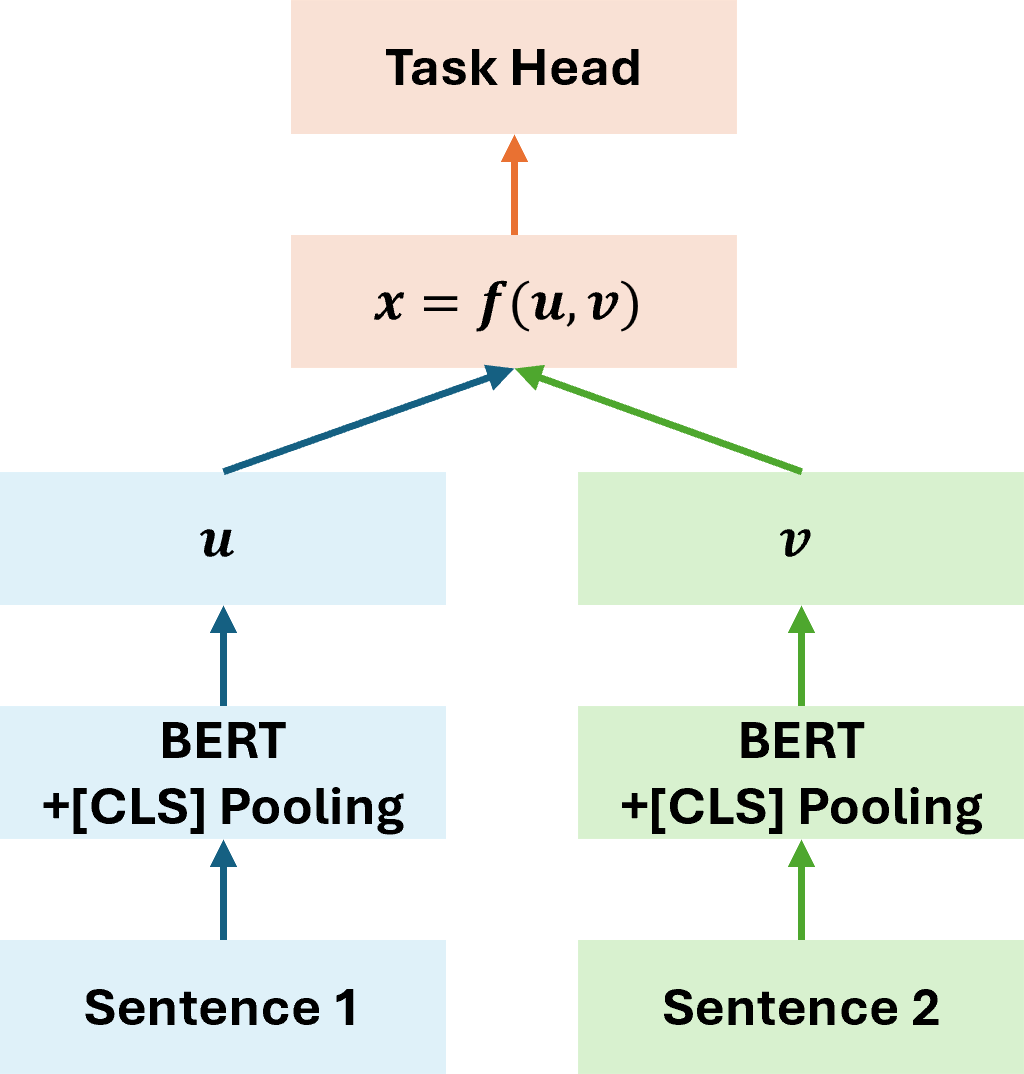
\includegraphics{pics/combine_1.png} }}%
          \qquad
          \subfloat[\centering Archetecture 2: Fused sentence embedding]
          {{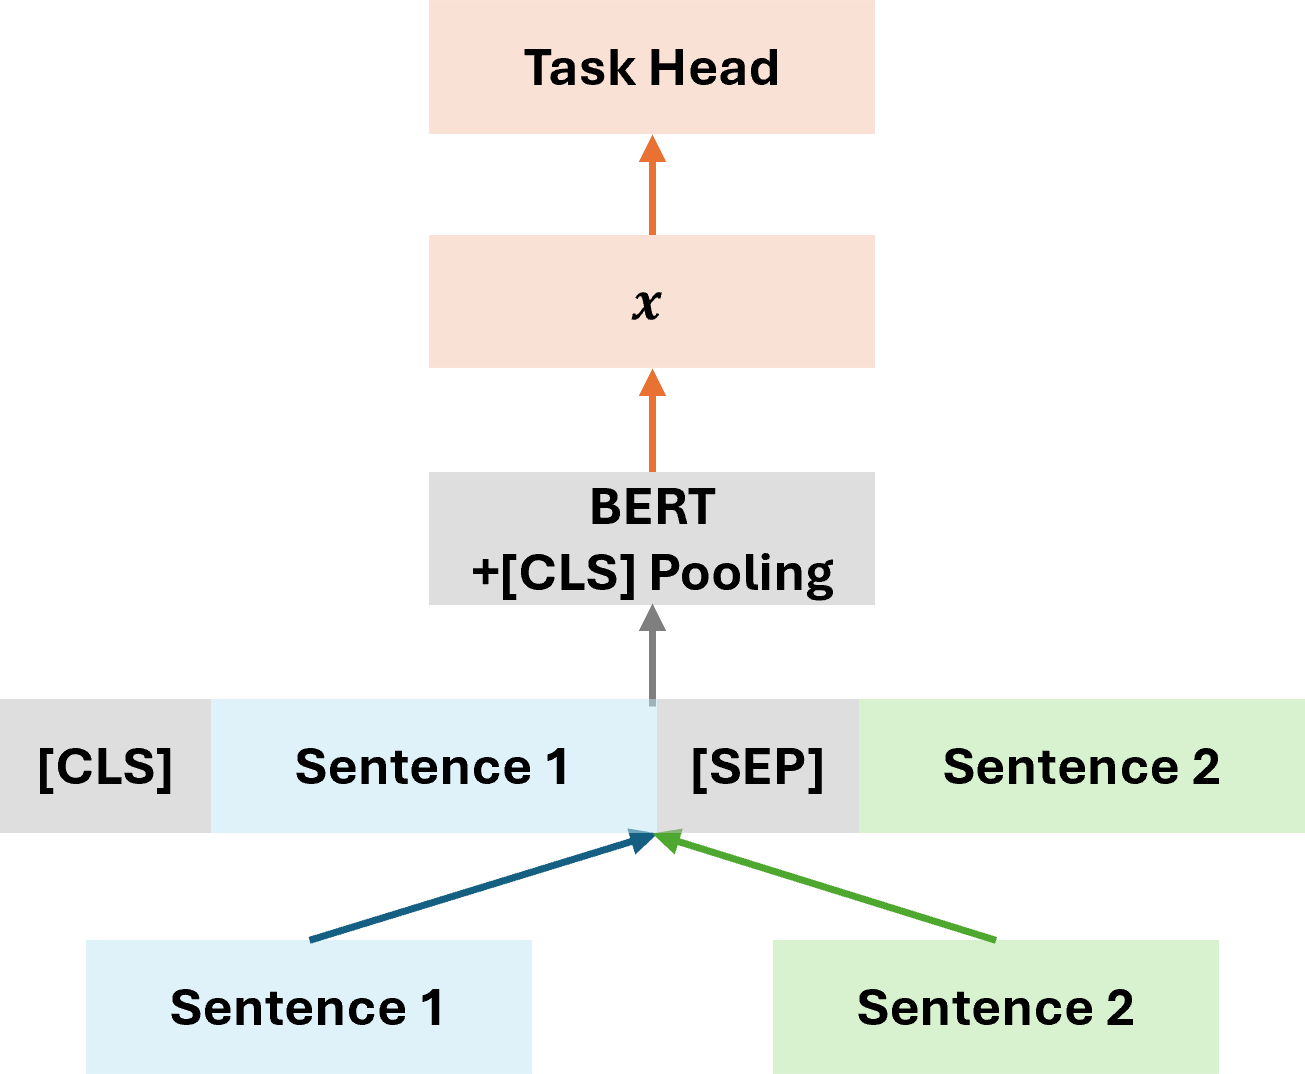
\includegraphics{pics/combine_2.png} }}%
          \caption{Two architectures for sentence-pair inputs: 
          (a) Each sentence is BERT-encoded separately, then pooled into a single embedding.
          (b) Sentence-pairs are concatenated with a \texttt{[SEP]} token and BERT-encoded into 
          one embedding.
          }%
          \label{fig:example}%
      \end{figure}

    \textbf{Baseline} Uses frozen pre-trained BERT\textsubscript{BASE} embeddings with a single linear projection layer as task head.

    \textbf{Combining Sentence Embeddings} (Figure \ref{fig:example})
    \begin{itemize}
        \item {Pooling Separate Embeddings:} Generates a joint embedding from two sentences encoded separately by BERT.
        \item {Fused Sentence Embedding:} Utilizes BERT's inherent training 
        with sentence pairs separated by the \texttt{[SEP]} token to encode sentence context 
        similarities.
    \end{itemize} 

    \textbf{Training Strategies}
    \begin{itemize}
        \item {Sequential Training:} Tasks are trained in succession 
        within each epoch. Specifically, model weights are updated per batch, with three tasks 
        forming a batch queue in the order of paraphrase detection, textual similarity, and 
        sentiment analysis.
        \item {Simultaneous Training:} Aggregates the losses for all tasks concurrently. 
        Each batch comprises three different tasks of the same batch size, and losses are 
        summed without weighting.
    \end{itemize}
    
  \end{block}

  % \begin{alertblock}{A highlighted block}
  % \end{alertblock}

\end{column}

\separatorcolumn

\begin{column}{\colwidth}

    \begin{block}{UDA Framework for Semi-Supervised Learning}
        \textbf{Advanced Data Augmentation} Generating augmented text for unlabeled datasets,
        via prompting LLaMA-3 Chat (8B) Model differently.
        \begin{itemize}
            \item Back-translation: Translates English sentences to French then back to English
            \item Sentence Completion: Completes sentence followed by "To put it differently,"
            \item Random-mask Completion: Completes randomly masked sentence with similar amount
            of words
        \end{itemize}

        \textbf{Training Signal Annealing (TSA)} Dynamically selects a subset of the labeled dataset at each training step $t$, we test linear, log, and exponential
        release schedule.
        Different threshold functions dictate the rate at which training signals of labeled examples are released.
        As shown in Figure 
        \ref{fig:tsa}, the TSA component proves effectiveness in mitigating overfitting during early epochs.
        \begin{figure}[H]%
          \centering
          \subfloat
          {{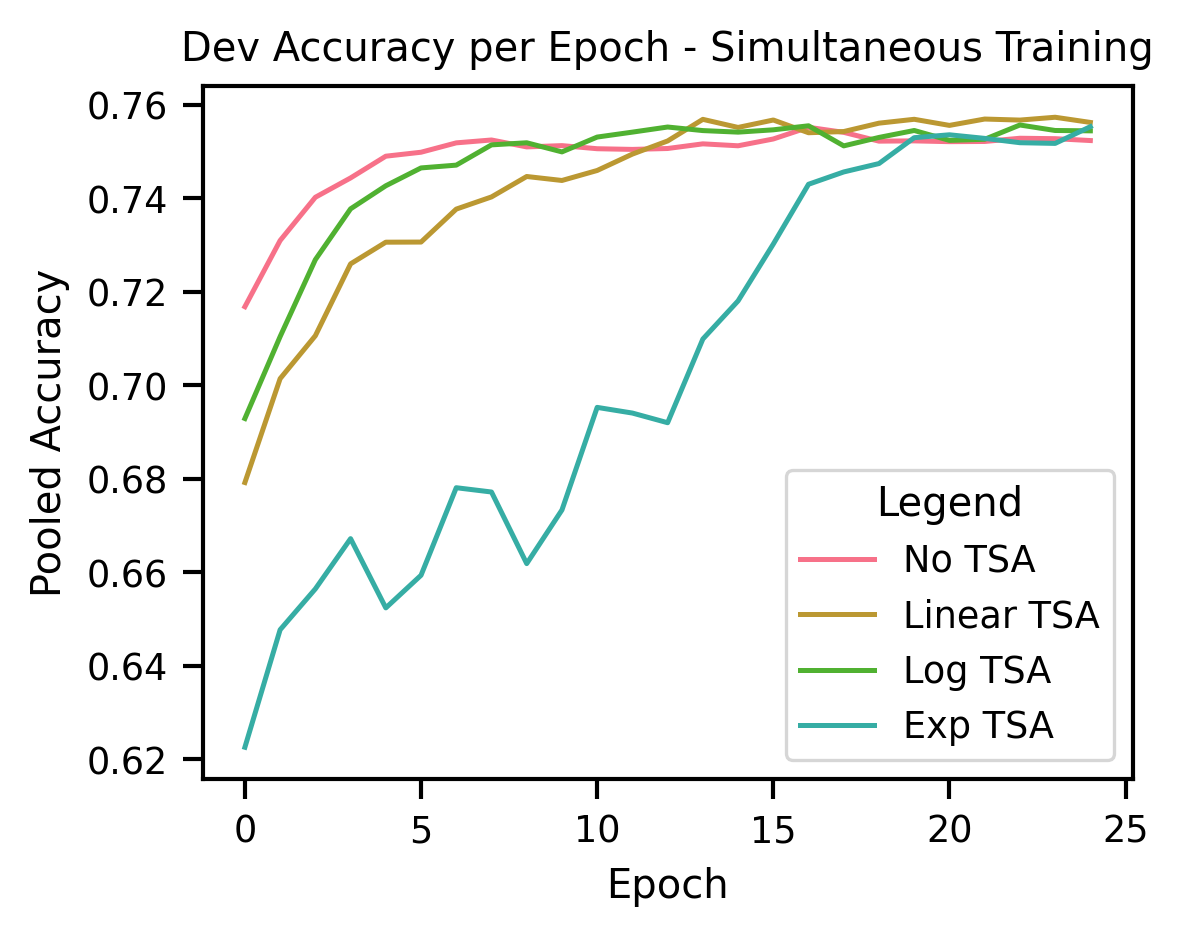
\includegraphics{pics/tsa-simul-dev.png} }}%
          \qquad
          \subfloat
          {{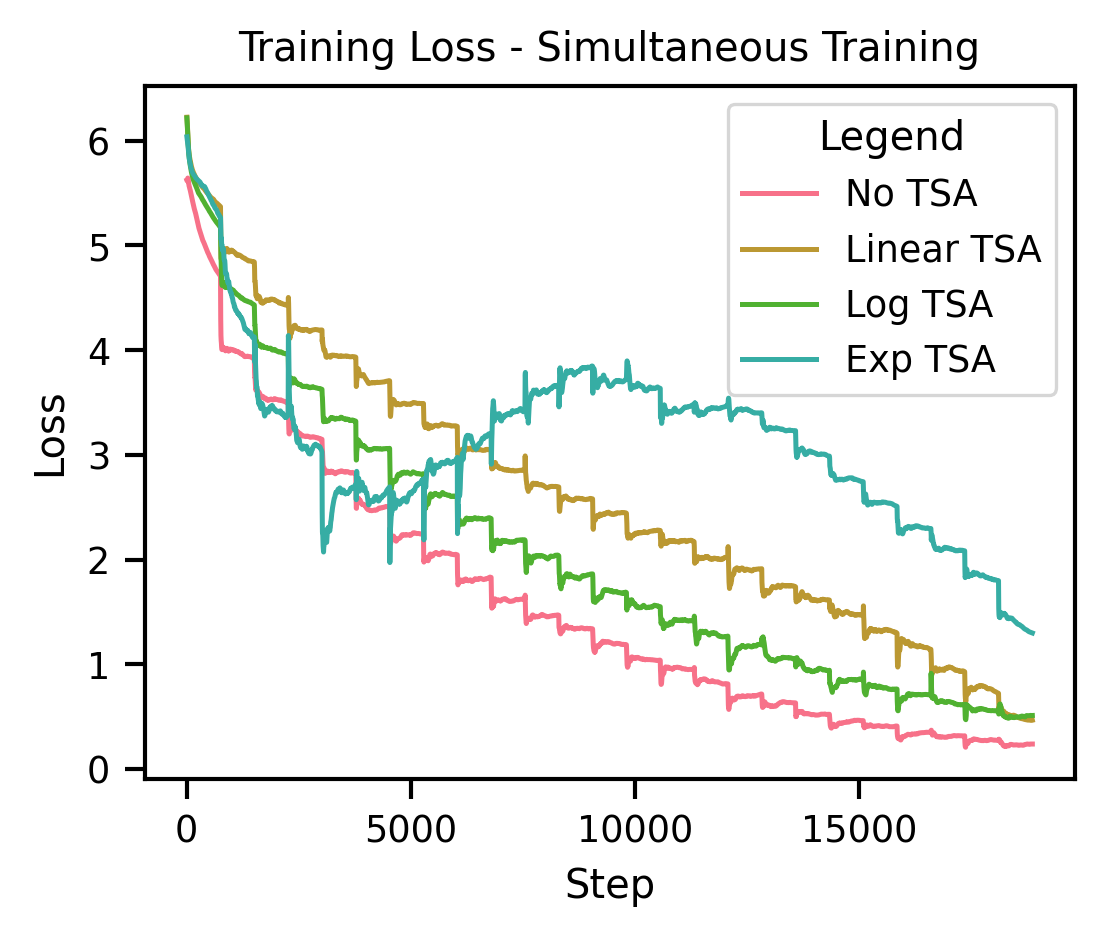
\includegraphics{pics/tsa-simul-loss.png} }}%
          \caption{Comparing characteristics of different TSA threshold functions}%
          \label{fig:tsa}%
        \end{figure}

        \textbf{Confidence Masking} To focus the unsupervised loss on distribution discrepancies arising from suboptimal data augmentation, we calculate the loss only on a subset of the unlabeled data where the model is confident in its prediction.

        \textbf{UDA Loss Function}
        Loss function is a combination of 
        supervised mean cross-entropy loss,
        and unsupervised mean KL-divergence loss between unsupervised and 
        augmented data.
        TSA and confidence masking is incorporated in UDA framework by dynamically 
        calculates loss on a subset of samples based on model performance.
        
        $$\mathcal{L} = 
        - \mathbb{E} \left[ \sum_{i=1}^{|L_t|} y_i \log p_{\theta}(x_i) \right]
        - \lambda \mathbb{E} \left[ \sum_{j=1}^{|U_t|} p_{\tilde{\theta}}(x_j) \log 
        \frac{p_{\tilde{\theta}}(x_j)}{p_{\theta}(\hat x_j)} \right]
        $$
    
    \end{block}

  \begin{block}{Results}
    The best performing model on dev set is using fused sentence embeddings +
    Linear TSA, training simultaneously. 
    \textbf{Our highest performing model has test set overall accuracy of 0.763, 
    0.517 on SST5, 0.839 on QQP, and 0.866 on STS separately.}
    \begin{table}[H]
      \centering
      \label{tab:baseline_ext}
      \begin{tabular}{@{}lcccc@{}}
        \toprule
        \textbf{Model} & \multicolumn{1}{c}{\textbf{SST5}} & \multicolumn{1}{c}{\textbf{QQP}} & \multicolumn{1}{c}{\textbf{STS}} & \multicolumn{1}{c}{\textbf{Acc}} \\ \midrule
        Baseline (last-layer only) & 0.309 & 0.667 & 0.209 & 0.527 \\
        Arc1-Simple Concat & 0.479 & 0.738 & 0.369 & 0.634 \\
        Arc1-Absolute difference & 0.510 & 0.733 & 0.532 & 0.670 \\
        Arc1-Dot Product Attention & 0.514 & 0.737 & 0.486 & 0.665 \\
        Arc2-Fused Sentence Embedding (BE) & 0.501 & 0.829 & 0.852 & 0.752 \\
        BE + Linear TSA & 0.520 & \textcolor{orange}{\textbf{0.836}} & 0.861 & \textcolor{orange}{\textbf{0.762}} \\
        BE + Linear TSA + UDA Back Translation & \textcolor{orange}{\textbf{0.520}} & 0.821 & \textcolor{orange}{\textbf{0.862}} & 0.758 \\
        BE + Linear TSA + UDA Sentence Completion & 0.506 & 0.820 & 0.853 & 0.751 \\
        BE + Linear TSA + UDA Random-mask Completion & 0.520 & 0.808 & 0.827 & 0.747 \\ 
        \bottomrule
      \end{tabular}
    \end{table}


  \end{block}

\end{column}

\separatorcolumn

\begin{column}{\colwidth}

  \begin{block}{Analysis}
    \begin{figure}[H]%
      \centering
      \subfloat[SST5 Dev Set Confusion Matrix normalized to predicted labels]
      {{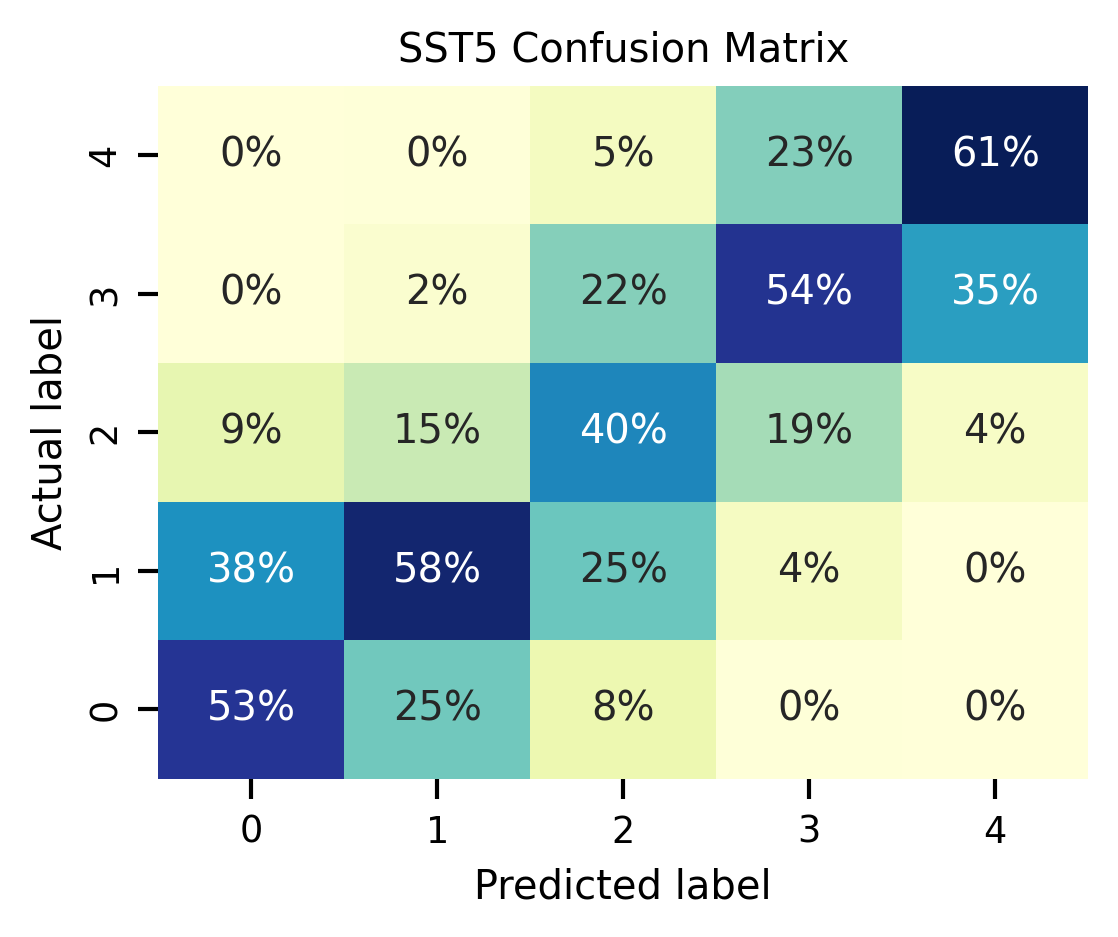
\includegraphics[width=0.3\textwidth]{pics/sst5.png} }}%
      \hfill
      \subfloat[QQP Dev Set Confusion Matrix normalized to predicted labels]
      {{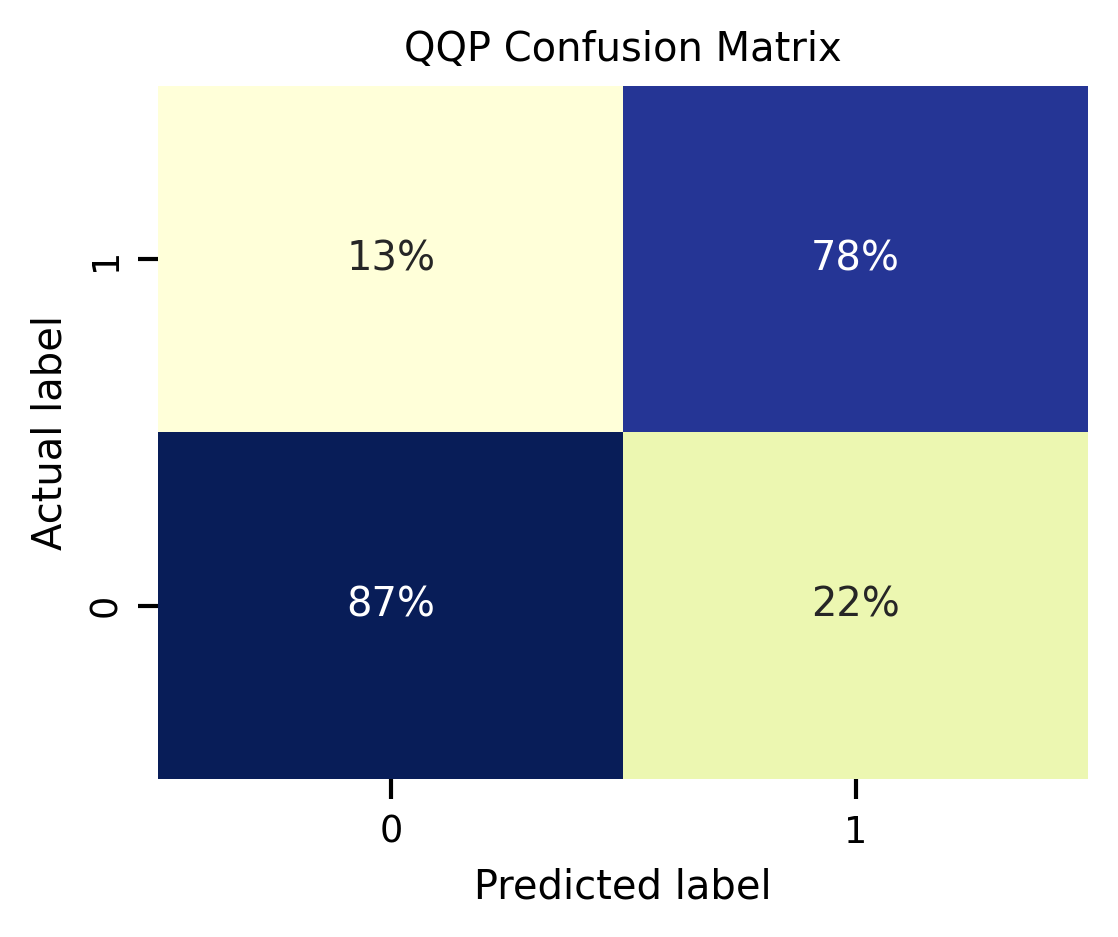
\includegraphics[width=0.3\textwidth]{pics/qqp.png} }}%
      \hfill
      \subfloat[STS Correlation Plot, line showing best fit]
      {{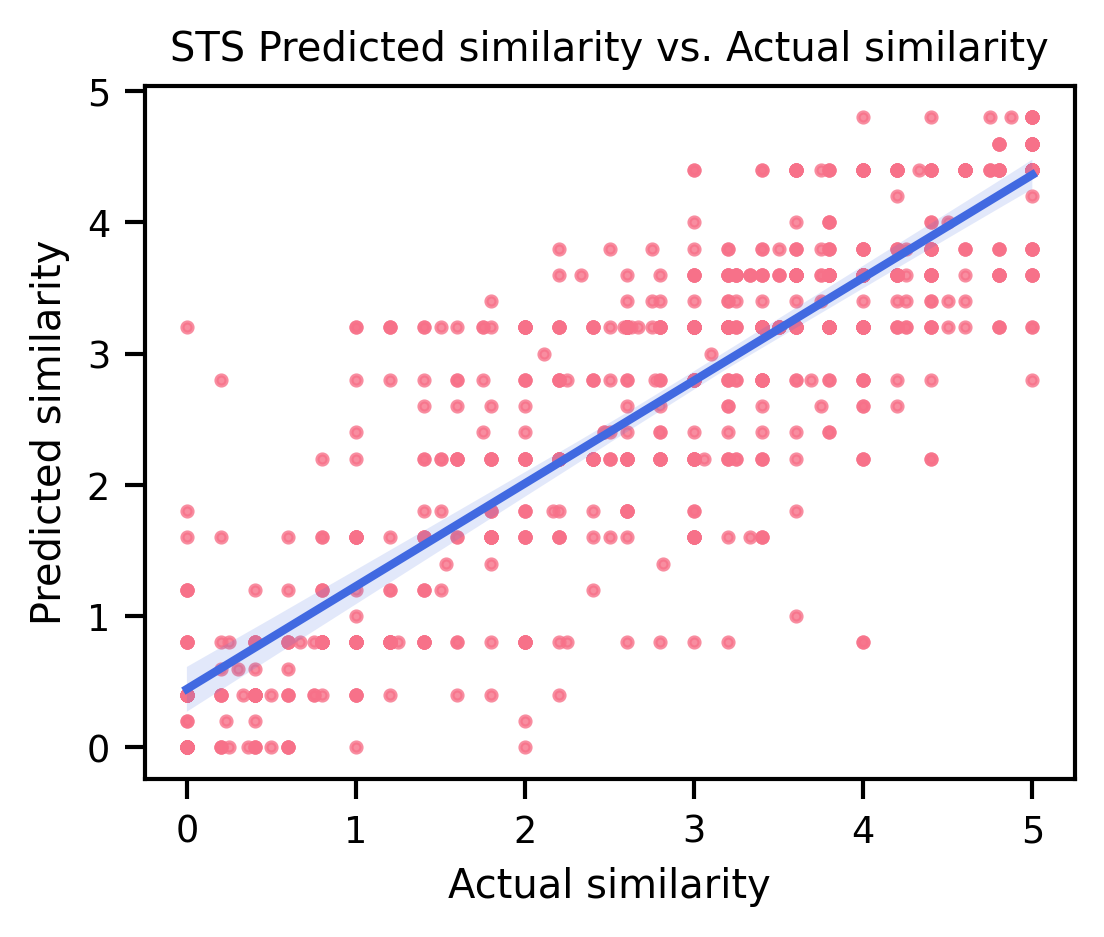
\includegraphics[width=0.3\textwidth]{pics/sts.png} }}%
      \caption{Analysis of Dev set performance of the model
      }%
      \label{fig:analysis}%
    \end{figure}
    In essence, the model exhibits a strong grasp of 
    sentiment analysis and sentence-pair similarity analysis.
    Mis-classifications primarily 
    occur between adjacent categories. Despite not explicitly training using an 
    ordinal categorical approach, the model effectively learns and interprets sentiment group
    relationship. On the hand, the model has challenges in:
    \begin{itemize}
        \item Fine-grained Sentiment Analysis SST5: Text ambiguities and human evaluator biases for neutral classes.
        \item Paraphrase Detection QQP: The model struggles with precision in positive class cases, especially when sentences have similar words in different orders or ambiguous human labels.
        \item Textual Similarity STS: The model tends to produce a narrower range of scores and has difficulty with extreme score assignments when sentences share common words.
    \end{itemize}
  \end{block}

  \begin{block}{Conclusion}
    \begin{itemize}
        \item \textbf{Key Findings:} Multitask learning strategies significantly enhance BERT’s performance across multiple NLP tasks. The fused sentence embedding approach combined with Linear TSA proves most effective.
        \item \textbf{Limitations:} Quality of data augmentation generated by LLaMA-3 has redundancy that undermines UDA's effectiveness.
        \item \textbf{Future Work:} Explore more efficient data augmentation techniques and advanced language features to further improve model robustness.
    \end{itemize}
  \end{block}

  \begin{block}{Ethics Statements}
    \begin{itemize}
        \item \textbf{Environmental impact:} UDA escalates 
        computational expenses due to generation of augmented datasets for large amount of unsupervised datasets via PLM prompts. Recent progress in few-shot and zero-shot learning with advanced PLMs suggests more efficient training paradigms.
        \item \textbf{Bias and toxicity amplification:} Existing biases or toxic language in training data and PLMs can be exacerbated in data augmentation 
        process. Employing existing models or APIs to scrutinize PLM-generated data can aid in filtering out 
        biased and toxic content and rephrasing biased text, thereby mitigating the amplification issue.
    \end{itemize} 
      
  \end{block}

  % \begin{block}{References}
  % \noindent\rule{\textwidth}{1pt}
  \heading{Reference}
  \bibliographystyle{plain}\bibliography{poster}
    % \nocite{*}
    % \footnotesize{}

  % \end{block}

\end{column}

\separatorcolumn
\end{columns}
\end{frame}

\end{document}
